\section{Behaviour}
\label{sec:behaviour}
We've chosen to use the goal driven behavior approach, because entities need to complete different actions to complete a goal. E.g., for a lumberjack to collect wood it needs to plan a path to the resource, then it needs to follow the path, once arrived it should start gathering, etc. Goal driven behavior provides a solid solution for these types of actions. Goals can be very large with loads off sub goals or actions, or they can be very small, this makes goal driven behavior easier extendable compared to state driven behavior for example. Since a goal can consist of multiple smaller goals, the Composite Pattern is a good solution to this problem. You can have small goals such as 'TraverseEdge' and also bigger goals like 'Work' and still treat them the same way. \cite{composite-pattern}

We created a single base class called Goal, which is a template class so that we can reuse it for different entity types. This class, together with the AtomicGoal and CompositeGoal classes, are shown in \cref{fig:goal}. Besides the Goal<T> class, we created two classes that inherit from it, the AtomicGoal and GoalComposite classes. The GoalComposite class contains a deque data structure that contains its subgoals. As you can see in \cref{fig:goal}, the GoalComposite<T> class also contains a couple of extra methods to add, remove, process and remove subgoals.

\subsection{Composite goals}
We created a couple of Composite goals for moving entities which we describe below. There is a class diagram \cref{fig:goalcomposite-inherit} in the appendix that illustrates the structure. This diagram doesn't show all composite goals, however it should give an impressions how we implemented this. 

\subsubsection{Think}
The Think goal is a goal that never gets removed. This goal is needed 
to determine an entity's next goal and activates that goal. It does so by 
calling the goals evaluator class, which returns a desirability value. The 
goal with the highest desirability gets chosen as the next goal. Desirability’s can be influenced by a variant of factors. E.g., how far away is the entity from an hostile entity. When there is an hostile enemy close it might not want to gather resources. Evaluators are a great way to create AI. Instead of using these evaluators we might use fuzzy logic. With fuzzy logic the actions of the entity should even feel more natural. 

\subsubsection{Follow Path}
\label{sec:followpath}
This goal traverses a path by adding the TraverseEdgeGoal class to its 
subgoals. This way a path consists of multiple instances of TraverseEdgeGoals
(\cref{sec:traverseedge}) which can be paused if the entity needs to do 
something else first, i.e. fleeing or resting. Once there are no more edges 
to traverse, this goal will be completed and removed from the entity's 
subgoals.

\subsubsection{Work}
This goal makes the entity go to the nearest resource to work. It first plans 
a path (\cref{sec:planpath}) to the nearest resource and then it follows that 
path (\cref{sec:followpath}). Once it arrives on the resource's location it 
starts to gather the resource (\cref{sec:gatherresource}). Once it's done 
gathering it plans another path, this time to the closest warehouse/depot. It follows 
this path and after it arrives it drops its resources 
(\cref{sec:dropresources}). Once all these goals are completed the work goal is completed as well.



\subsection{Atomic goals}
Besides Composite goals, we also have Atomic goals. You can compare Atomic 
goals with leaf nodes of a tree structure. Atomic goals are the actual actions
 that an entity needs to do. As shown in \cref{fig:atomicgoal-inherit}, an atomic 
 goal has no subgoals. Calling the AtomicGoal::add\_subgoal() method results in an 
 exception.
 
 \begin{figure}[!htb]
    \centering
    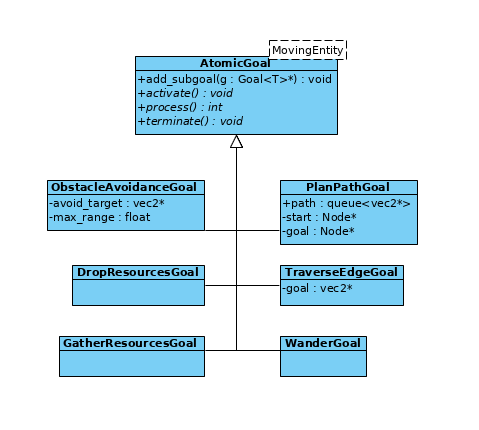
\includegraphics{res/AtomicGoal-Inherit.jpg}
    \caption{AtomicGoal Inheritance.}\label{fig:atomicgoal-inherit}
\end{figure}

\subsubsection{Wander}
The wandering goal is another goal that never gets removed, just like the 
think goal. An entity always needs to wander around if it has absolutely 
nothing to do. The only thing this goal does is activate the wander steering 
behaviour (\cref{sec:wander}).

\subsubsection{Obstacle Avoidance}
The obstacle avoidance goal activates the obstacle avoidance steering 
behaviour. When this goal is activated, it adds the steering behaviour to the 
entity's behaviours. Once the distance to the target that it needs to avoid 
is big enough, the goal is completed and the steering behaviour also gets 
removed from the entity.

\subsubsection{Drop Resources}
\label{sec:dropresources}
Once an entity has gathered enough resources, it needs to drop them at a 
warehouse/depot. This goal simply removes the resources the entity gathered and adds them to the resources of the player. When it dropped all of it's resources at the warehouse, the goal is completed.

\subsubsection{Gather Resource}
\label{sec:gatherresource}
This goal calls the Gather() method from a resource entity. This method extracts resources from the resource entity and adds it to the entity that is gathering the resource. Once the resource entity has been depleted or the maximum carrying capacity of the gathering entity has been reached this goal will be completed.

\subsubsection{Plan Path}
\label{sec:planpath}
The plan path goal plans a path using the A* algorithm, using the Manhattan 
heuristic (\cref{sec:pathplanning}). Once the path has been generated, it gets set as the active path 
for the given entity. This is the only task it needs to complete before 
getting removed from the containing goal.

\subsubsection{Traverse Edge}
\label{sec:traverseedge}
This goal uses the Seek behaviour explained in \cref{sec:seek-behaviour}. Once 
this class gets instantiated it adds an instance of SeekStrategy to the 
entity's behaviour. The only thing it needs to do while processing, is 
to check whether the entity has this behaviour, and if so if it's close 
enough to the next node on the graph. If it's close enough, the goal has been 
completed.


\newpage

